\subsection{Business Case}
\subsubsection{Den nuværende situation}
\subparagraph{Timeregistrering til regning}

    Hver fredag udfylder svendene en papirsskabelon, hvor de skriver stedet arbejdet er blevet udført, hvilken dag arbejdet er udført, hvad der er gjort, hvilke materialer der er taget fra firmaets eget værksted, og hvor mange timer der er brugt.
    Dette gøres for alle timerne i ugen.
    
    Hver tirsdag eller onsdag samler sekretæren alle deres registreringer og skriver regninger til Halvorsen's kunder.

\subparagraph{Timeregistrering til aflønning}
    Hver anden fredag udfylder svendene også en anden papirsskabelon, hvor de skriver for alle 14 dage. De skriver, hvor mange timer de har arbejdet de enkelte dage, og overarbejdstimer skrives separat.
    
    For både regning og aflønningstimeregistreringen er svendene derfor nød til at køre tilbage på værkstedet for at udfylde papirerne.

Et BPMN diagram over begge processer kan ses på figur \ref{fig:BPMN}.
    
\begin{figure}[h]
    \makebox[\textwidth][c]{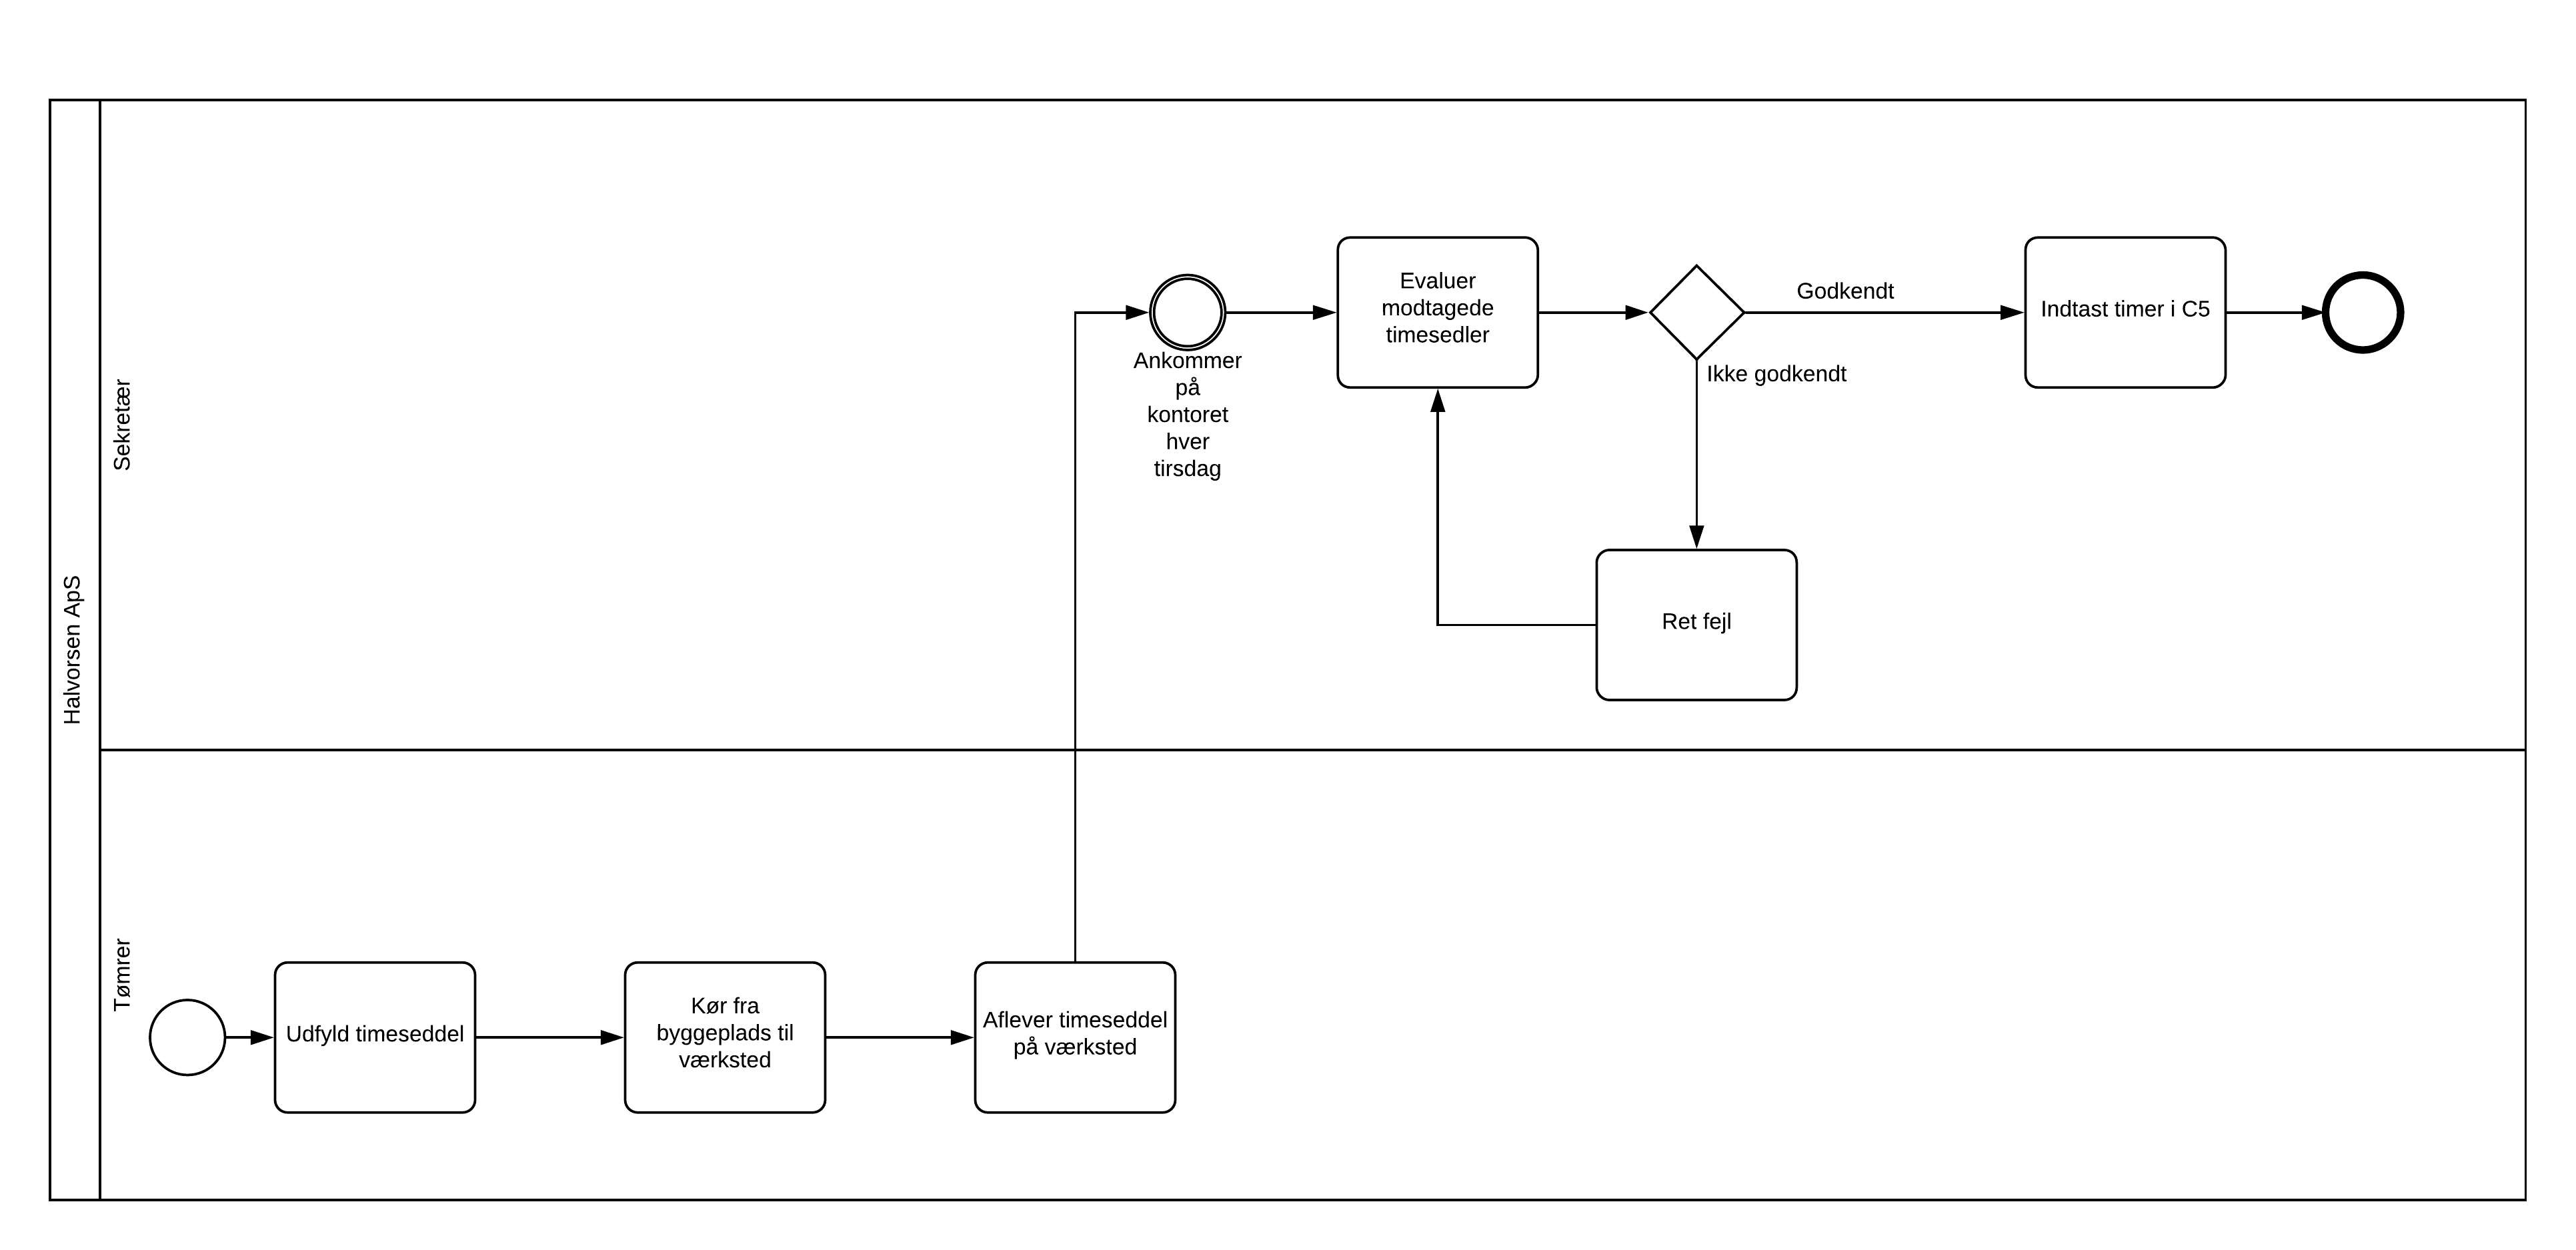
\includegraphics[scale = 0.6]{BPMN.png}}
    \caption{BPMN for tidsregistrering}
    \label{fig:BPMN}
\end{figure}
    
\subparagraph{Intern materialebestilling}
    Når en svend opdager, at der mangler materialer på en byggeplads, som de skal bruge, ringer de hjem til tømmermesteren. De fortæller, hvad de skal bruge, de specifikke mål, samt hvor og hvornår det skal bruges.
    
    Derfor skal Torben selv huske på alle bestillingerne. Det kan give problemer, da det er nemt at glemme et specifikt mål, eller Torben kan høre forkert.
    
\subparagraph{Arbejdstegninger}
    Svendene har arbejdstegninger i papirform med i deres biler ud på byggepladserne.
Det betyder, at over tid bliver tegningerne krøllede og beskidte.
Der er heller ikke mulighed for at forstørre en lille del op, så man nemmere kan se præcis, hvad der står på tegningen.
De har prøvet at laminere tegningerne, men så kan de ikke foldes sammen og være i en lomme.
    
\subsubsection{Formålet med projektet}
    Projektet skal effektivisere den interne kommunikation i     firmaet.
    Denne rapport arbejder med at effektivisere timeregistreringen.
    
   Projektet skal sørge for, at tidsregistreringen kan foregå andre steder end hjemme på værksedet og derved spare kørselstid.
   Projektet skal også være med til at minimere antallet af tidsregistreringsfejl og derved effektivisere sekretærens tid på kontoret.
    
\subsubsection{Løsningsscenarier}

\begin{table}[H]
\centering
\makebox[\textwidth][c]{
\begin{tabular}{@{}cl@{}}
\toprule
\textbf{Fordele}                                                                                                                         & \multicolumn{1}{c}{\textbf{Ulemper}}                                                                                                                          \\ \midrule
\multicolumn{2}{|c|}{\textbf{Fortsæt som normalt(0 - scenarie)}}                                                                                                                                                                                                                                                       \\ \midrule
\multicolumn{1}{|l|}{\begin{tabular}[c]{@{}l@{}}Ingen ekstra udgifter\\ Ingen omstillingsperiode\end{tabular}}                         & \multicolumn{1}{l|}{\begin{tabular}[c]{@{}l@{}}Ingen optimering ved hjælp af IT.\\ Hyppige menneskelige fejl.\end{tabular}}                                                                                                        \\ \midrule
\multicolumn{2}{|c|}{\textbf{Køb af allerede eksisterende løsning f.eks Navision(1 - scenarie)}}                                                                                                                                                                                                                       \\ \midrule
\multicolumn{1}{|l|}{\begin{tabular}[c]{@{}l@{}}Løsningen eksistere allerede\\ Mulighed for køb af support\end{tabular}}               & \multicolumn{1}{l|}{\begin{tabular}[c]{@{}l@{}}Stejl indlæringskurve\\ Dyr løsning\end{tabular}}                                  \\ \midrule
\multicolumn{2}{|c|}{\textbf{Email skabelon(1 - scenarie)}}                                                                                                                                                                                                                                                            \\ \midrule
\multicolumn{1}{|l|}{Simpelt at sætte op}                                                                                                & \multicolumn{1}{l|}{\begin{tabular}[c]{@{}l@{}} Stor risiko for menneskelige fejl.\end{tabular}}                                  \\ \midrule
\multicolumn{2}{|c|}{\textbf{\begin{tabular}[c]{@{}c@{}}App til Smartphone og Tablet(1 - scenarie)\\ (Den valgte løsning)\end{tabular}}}                                                                                                                                                                               \\ \midrule
\multicolumn{1}{|l|}{\begin{tabular}[c]{@{}l@{}}Løsningen kan skræddersyes og udvides\\ til at opfylde virksomhedens krav.\end{tabular}} & \multicolumn{1}{l|}{\begin{tabular}[c]{@{}l@{}}De er nød til at anskaffe endten arbejdstelefoner\\ til medarbejderne eller tablets til hver bil.\end{tabular}} \\ \bottomrule
\end{tabular}
}
\end{table}

\subsubsection{Gevinstanalyse}
\subparagraph{Strategi for gevinstrealisering}
Vi ønsker at optimere tidsforbrug i forbindelse med intern kommunikation. Derved skal der være mulighed for, at brugere af programmet kan spare tid ved timeregistrering, intern materialebestilling og behandling af arbejdstegninger.

Under udarbejdelsen af systemet er det meget vigtigt, at vi sørger for, at systemet er så nemt at bruge som muligt, da, som vi beskriver nærmere i afsnit \ref{interessent}, vil næsten alle brugere af systemet være teknisk uerfarne.

Derudover er det vigtigt, at de data, systemet gemmer, er præcise, da det er data der vil blive sendt regninger og lønsedler ud fra.

Gevinsten af projektet er effektivisering, da der vil blive sparet tid ved at undgå kørsel tilbage på kontoret.

\subparagraph{Effektiviseringsgevinster}
Ved at kigge på BPMN'en beskrevet i figur \ref{fig:BPMN} og fjerne nødvendigheden for at køre fra byggeplads til værksted vil hver tømrer spare 30 minutters ekstra kørsel hver fredag.
Og hvis man også kan fjerne nødvendigheden for, at sekretæren skal rette fejl i timesedlerne, vil BPMN'en for den nye situation se ud som på figur \ref{fig:BPMN2}.

\begin{figure}
    \makebox[\textwidth][c]{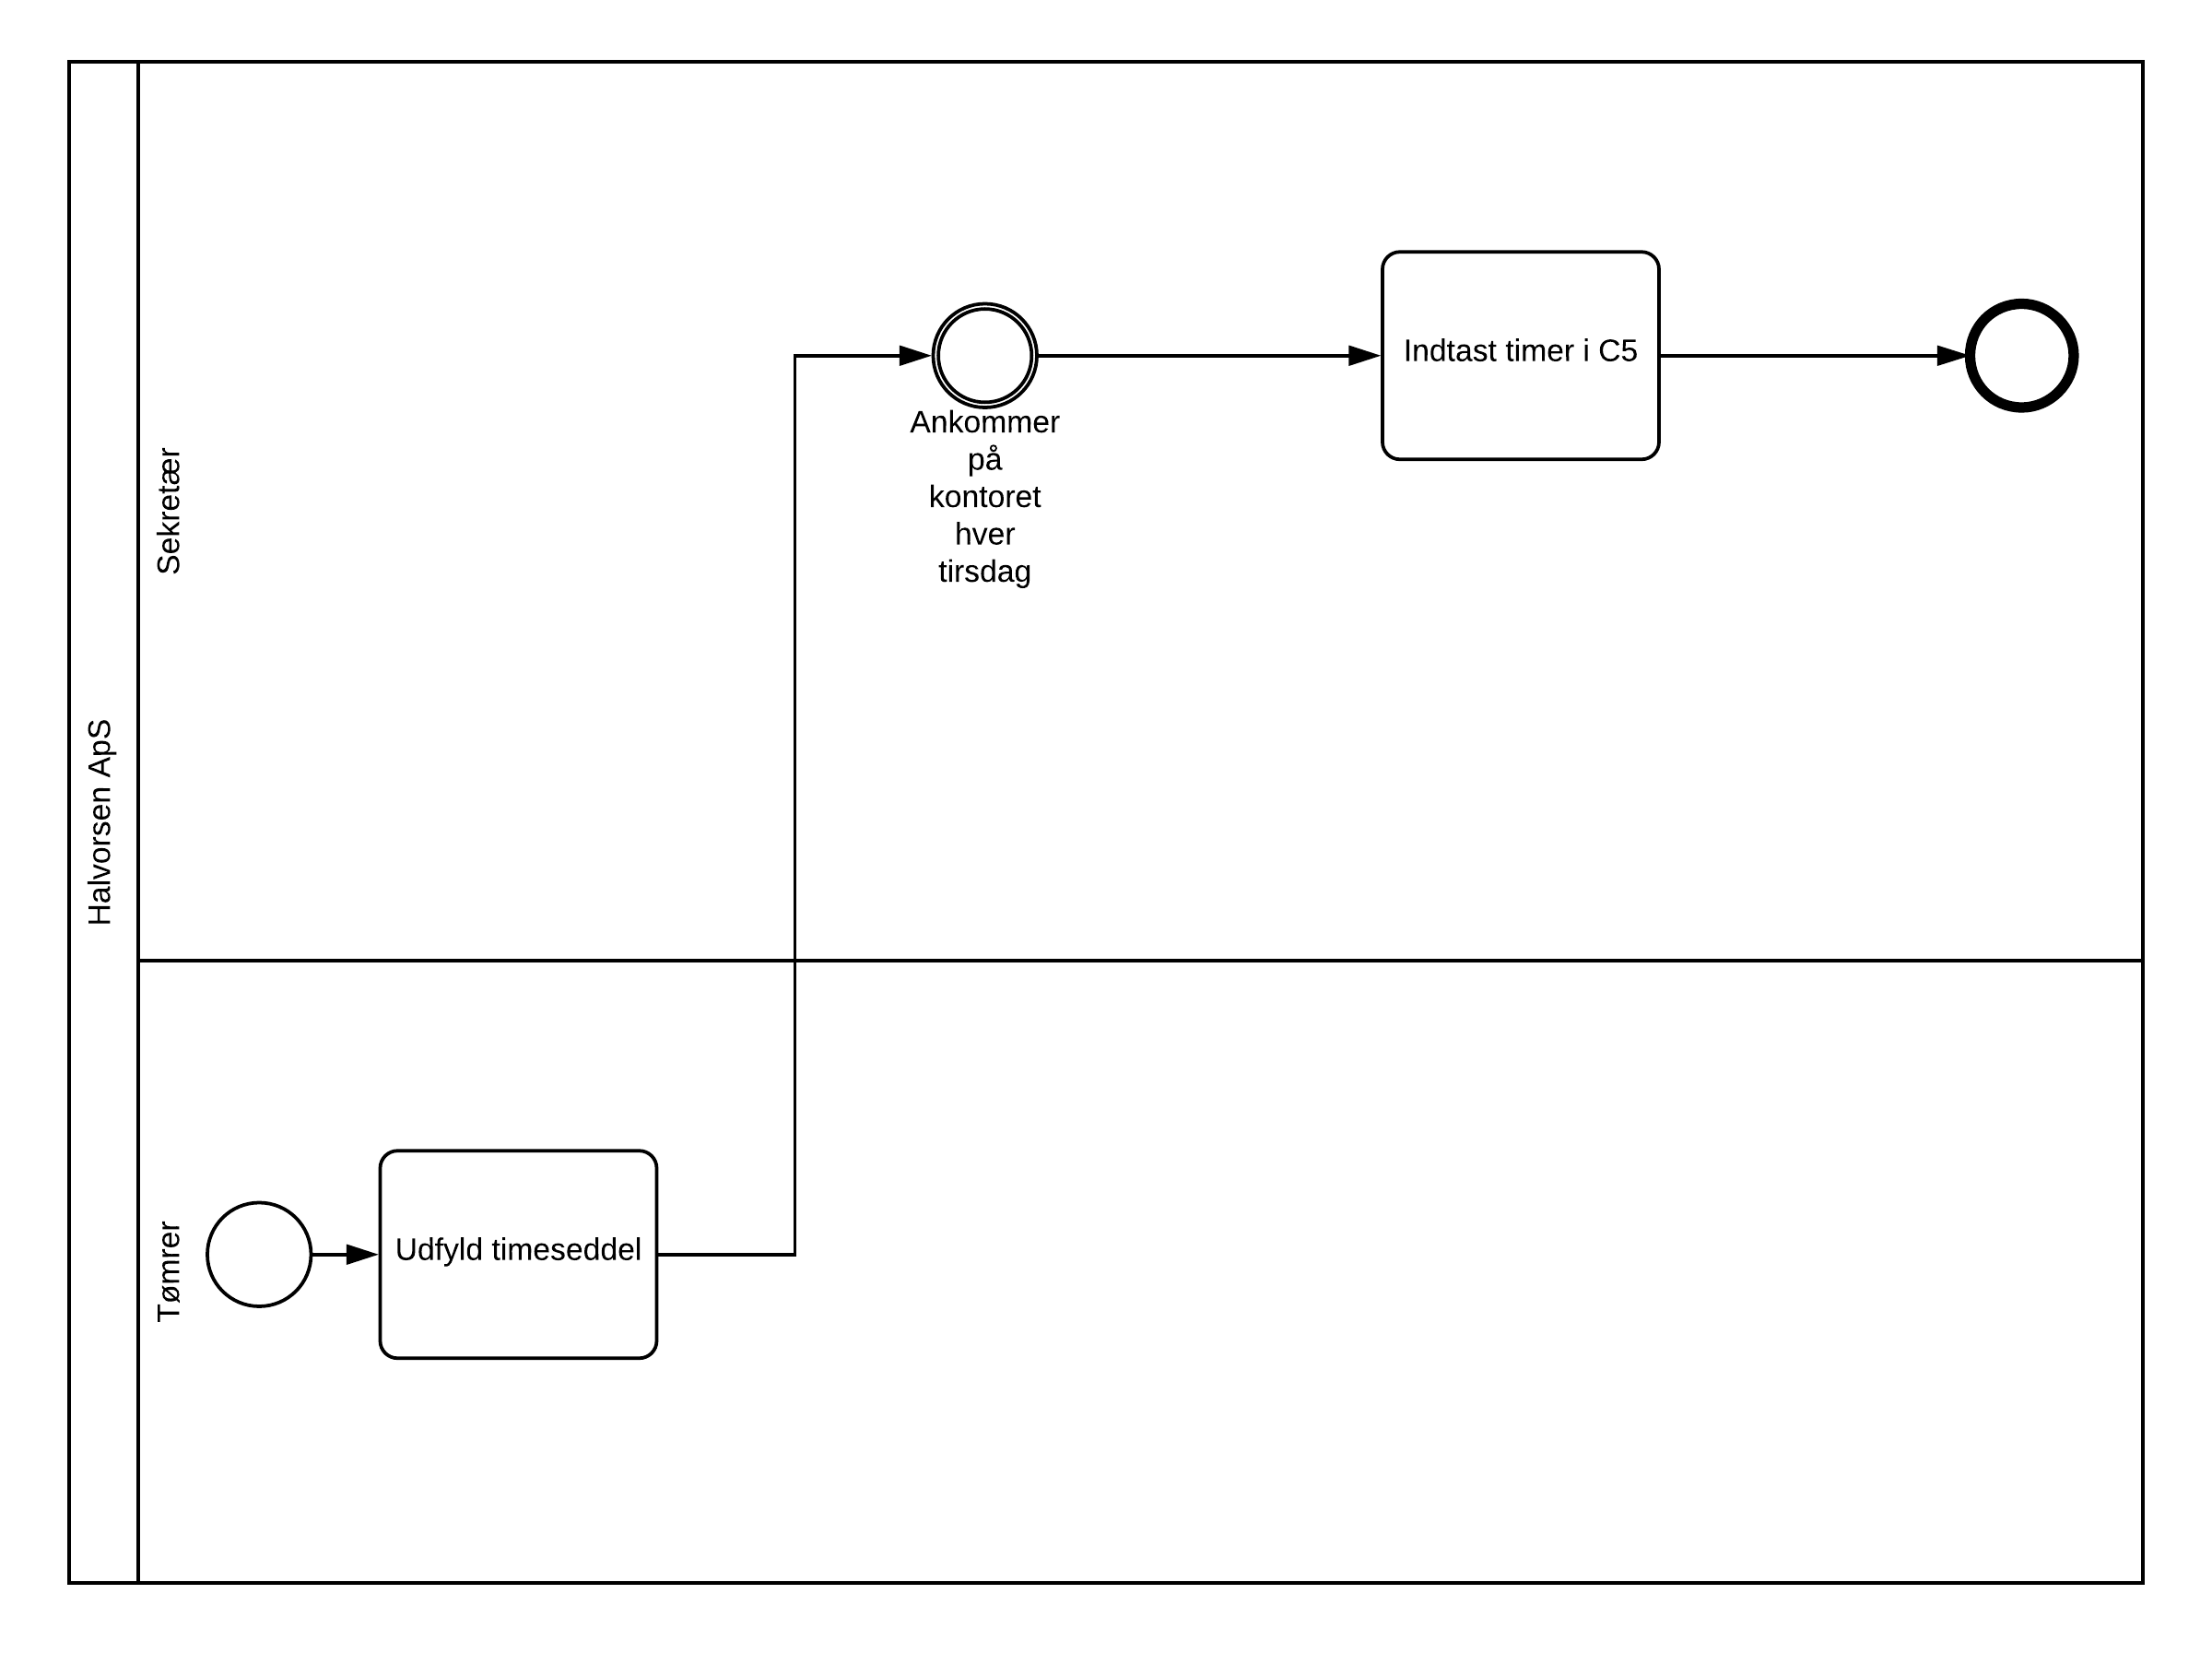
\includegraphics[scale = .6]{BPMN2.png}}
    \caption{BPMN for tidsregistrering}
    \label{fig:BPMN2}
\end{figure}

\subparagraph{KPI}
Da formålet med løsningen er at spare tid er følgende KPI blevet sat op, så besparelsen kan måles:

\begin{table}[H]
\makebox[\textwidth][c]{
\begin{tabular}{|l|l|}
\hline
KPI                                                                                            & Antal timer sparet ved tidsregistrering.               \\ \hline
Hvorfor måles?                                                                                 & For at kunne kvanticere løsningens effektivitet.       \\ \hline
Hvordan måles?                                                                                 & Måles med et stopur.                                   \\ \hline
Hvem er ansvarlig for målingen?                                                                & Sekretær og Tømrermester                               \\ \hline
Forventet målingsdato?                                                                         & Hver fredag, når der tidsregistreres.                  \\ \hline
Forventet værdiinterval for måling                                                             & 2-5 minutter.                                          \\ \hline
Måling                                                                                         & Ikke udført.                                           \\ \hline
\begin{tabular}[c]{@{}l@{}}Handlingsplan i fald måling\\ ligger uden for interval\end{tabular} & Opdater programmet, så det er mere effektivt at bruge. \\ \hline
Ansvarlig for handling                                                                         & Tømrermester                                           \\ \hline
\end{tabular}
}
\end{table}

Desværre er vi først blevet opmærksomme på, at vi burde lave en KPI sent i projektforløbet, og derfor har vi ikke nået at udføre nogen målinger.

Det er ærgeligt, og vi har alle taget det med som erfaringer til videre projekter.

\subsubsection{Interessentanalyse}\label{interessent}
Mette og tømrermesteren Torben er som sekretær og tømrermester samt virksomhedsledere involveret i udviklingen af produktet.
Især Mette, da hun skal bruge programmet til bogholderi.
Og Torben skal bruge det til det daglige arbejde på samme måde som hans tømrersvende.

Tømrerne skal også involveres i projektet, eftersom programmet skal bruges af dem og løsningen omhandler dem.

For både Torben og hans svende gælder det, at de alle er en del af den ældre generation, og de derfor ikke er vokset op med IT systemer som en fast del af deres hverdag.
Derfor er det vigtigt, at løsningen er intuitiv og nem at bruge for dem, ellers er det ikke muligt for systemet at optimere deres hverdag.

Vi mener ikke, at der er nogen, der direkte er modstandere af systemet, da målet er at gøre det nemmere for tømrerne.